\documentclass[12pt,a4paper,twoside]{book}
\usepackage[margin=1in]{geometry}
\usepackage[utf8]{inputenc}
\usepackage[dutch, english]{babel}
\usepackage[T1]{fontenc}
\usepackage{afterpage}
\usepackage{amsmath}
\usepackage{amssymb}
\usepackage{amsthm}
\usepackage{algorithm}
\usepackage[noend]{algpseudocode}
\usepackage[page]{appendix}
\usepackage{biblatex}
\usepackage{caption}
\usepackage{fancyhdr}
\usepackage{float}
\usepackage{fontawesome5}
\usepackage[final]{hyperref}
\usepackage[acronym,automake,section]{glossaries}
\usepackage{lipsum}
\usepackage{listing}
\usepackage{listings,lstautogobble}
\usepackage[default,scale=0.95]{opensans}
\usepackage[nottoc]{tocbibind}
\usepackage{pdfpages}
\usepackage{setspace}
\usepackage[detect-weight=true, binary-units=true, range-phrase=-]{siunitx}
\usepackage[caption=false]{subfig}
\usepackage{tabularx}
\usepackage{textcomp}
\usepackage{tikz}
\usepackage{tikzscale}
\usepackage{titlesec}
\usepackage{draftwatermark}
\usepackage{cleveref}

% Tikz libraries.
\usetikzlibrary{arrows,arrows.meta,automata,calc,shapes.geometric,positioning}

% Watermark.
\SetWatermarkText{Draft}
\SetWatermarkScale{1.5}
\SetWatermarkColor[rgb]{0.95,0.95,0.95}

% Blank pages.
\newcommand\blankpage{%
	\null
	\thispagestyle{empty}%
	\addtocounter{page}{-1}%
	\newpage}

% Chapters.
\titleclass{\chapter}{straight}
\titleformat{\chapter}[display]{\normalfont\huge\bfseries}{\chaptertitlename\ \thechapter}{18pt}{\huge}
\titlespacing*{\chapter}{0pt}{20pt}{20pt}

\renewcommand{\chaptermark}[1]{\markright{\MakeUppercase{#1}}}
\renewcommand{\sectionmark}[1]{\markright{\thesection~#1}}

\newcommand{\headerfmt}[1]{\textsl{\textsf{#1}}}
\newcommand{\headerfmtpage}[1]{\textsf{#1}}

% Header/footer.
\fancyhf{}
\fancyhead[LE,RO]{\headerfmtpage{\thepage}}
\fancyhead[LO]{\headerfmt{\rightmark}}
\fancyhead[RE]{\headerfmt{\leftmark}}
\renewcommand{\headrulewidth}{0.5pt}
\renewcommand{\footrulewidth}{0pt}

\fancypagestyle{plain}{
	\fancyhf{}
	\fancyhead[LE,RO]{\headerfmtpage{\thepage}}
	\fancyhead[LO]{\headerfmt{\rightmark}}
	\fancyhead[RE]{\headerfmt{\leftmark}}
	\renewcommand{\headrulewidth}{0.5pt}
	\renewcommand{\footrulewidth}{0pt}
}

% Colours.
\definecolor{black}{RGB}{0, 0, 0}
\definecolor{bisque}{HTML}{FFE4C4}
\definecolor{code-background}{HTML}{EEEEEE}
\definecolor{code-delim}{RGB}{20,105,176}
\definecolor{darkgray}{rgb}{.4,.4,.4}
\definecolor{groovyblue}{HTML}{0000A0}
\definecolor{groovygreen}{HTML}{008000}
\colorlet{code-punct}{red!60!black}
\definecolor{ugent-blue}{RGB}{30, 100, 200}

% Meta-information.
\hypersetup{
	pdfauthor = {Pieter De Clercq},
	pdftitle = {Optimising Continuous Integration using Test Case Prioritisation},
	pdfsubject = {Master's dissertation submitted in order to obtain the academic degree of Master of Science in Computer Science, june 2020},
	linkcolor = black,
	citecolor = ugent-blue,
	urlcolor = ugent-blue,
	colorlinks = true,
}

% Mathematical definitions.
\theoremstyle{break}
\newtheorem{definition}{Definition}

\lstset{
	numbers=left,
	numberstyle=\scriptsize,
	stepnumber=1,
	numbersep=8pt,
	showstringspaces=false,
	breaklines=true,
	frame=lines,
	captionpos=b,
	backgroundcolor=\color{code-background},
	autogobble=true,
    escapeinside={(*}{*)},
    upquote=true
}

% Code listings.
\lstdefinelanguage{Groovy}[]{Java}{
	keywords=[9]{buildscript, dependencies, classpath, apply, plugin, velocity, base, repository, server}
}

\renewcommand{\lstlistingname}{Example}
\renewcommand{\lstlistlistingname}{List of \lstlistingname s}

% Table columns.
\newcolumntype{C}{>{\centering\arraybackslash}X}

% Pseudocode keywords.
\renewcommand{\algorithmicrequire}{\textbf{Input:}}
\renewcommand{\algorithmicensure}{\textbf{Output:}}

% Add the references resource.
\addbibresource{references.bib}

\makeglossaries

% Macro's
\newcommand{\CI}{Continuous Integration}
\newcommand{\github}{GitHub}
\newcommand{\githubactions}{GitHub Actions}
\newcommand{\gitlab}{GitLab}
\newcommand{\gitlabci}{GitLab CI}
\newcommand{\junit}{JUnit}
\newcommand{\travisci}{Travis CI}
\newcommand{\tcp}{Test Case Prioritisation}
\newcommand{\tcs}{Test Case Selection}
\newcommand{\tsm}{Test Suite Minimisation}
\newcommand{\vcs}{Version Control System}
\newcommand{\velocity}{VeloCIty}
\newcommand{\bolditem}[1]{\item \textbf{#1:}}

% Acronyms.
\newacronym{ci}{CI}{\CI}
\newacronym{ieee}{IEEE}{The Institute of Electrical and Electronics Engineers}
\newacronym{sdlc}{SDLC}{Software Development Life Cycle}
\newacronym{tcp}{TCP}{\tcp}
\newacronym{tcs}{TCS}{\tcs}
\newacronym{tdd}{TDD}{Test-driven development}
\newacronym{tsm}{TSM}{\tsm}
\newacronym{vcs}{VCS}{\vcs}

% Fix hyphenation.
\brokenpenalty=1000
\babelhyphenation[dutch]{Java}
\babelhyphenation[dutch]{Python}
\babelhyphenation[dutch]{VeloCIty}
\babelhyphenation[english]{Java}
\babelhyphenation[english]{Python}
\babelhyphenation[english]{VeloCIty}

% Glossary items.
\newglossaryentry{mapreduce}{name={MapReduce},description={a programming paradigm that allows large amounts of data to be processed in a distributed manner}}
\newglossaryentry{rest}{name={REST},description={Representational State Transfer is an architectural design pattern used by modern web applications. This design pattern encourages standardised communication using existing HTTP methods}}
\newglossaryentry{regression}{name={regression},description={a feature that was once working as intended but is suddenly malfunctioning}}
\newglossaryentry{testsuite}{name={test suite},description={the collection of all test cases in an application}}
\newglossaryentry{blackboxtest}{name={black-box test},description={a test case that was constructed without any knowledge of the function(s) under test}}
\newglossaryentry{whiteboxtest}{name={white-box test},description={a test case that was constructed after fully inspecting the function(s) under test}}

% References.
\crefname{listing}{example}{examples}  
\Crefname{listing}{Example}{Examples}

\begin{document}
\onehalfspacing
	
% Titlepage.
\frontmatter
\pagestyle{empty}
%\includepdf[pages=-]{titlepage.pdf}

%\blankpage{}

% Admission.
%% !TeX root = thesis.tex

\chapter*{Admission}
\selectlanguage{english}
\noindent The author gives the permission to use this thesis for consultation and to copy parts of this thesis for personal use. Every other use is subject to the copyright laws, more specifically the source must be extensively specified when using results from this thesis.\\

\selectlanguage{dutch}
\noindent De auteur geeft de toelating deze masterproef voor consultatie beschikbaar te stellen en delen van de masterproef te kopi\"eren voor persoonlijk gebruik. Elk ander gebruik valt onder de bepalingen van het auteursrecht, in het bijzonder met betrekking tot de verplichting de bron uitdrukkelijk te vermelden bij het aanhalen van resultaten uit deze masterproef.\\

\selectlanguage{english}

\noindent Pieter De Clercq -- \today.
\clearpage

% Acknowledgements.
%% !TeX root = thesis.tex

\chapter*{Acknowledgements}

Completing this thesis would not have been possible without the help and support of many people, some of which I want to thank personally.\\

\noindent First of all, I want to thank prof. dr. Bruno Volckaert and prof. dr. ir. Filip De Turck for allowing me to propose this subject and for their prompt and clear responses to every question I have asked. I especially want to thank you for permitting me to insert a two-week hiatus during the Easter break, so I could help out on the UGent Dodona project.\\

\noindent Secondly, I want to express my gratitude towards my counsellors Jasper Vaneessen and Dwight Kerkhove, for steering me into researching this topic, as well as their guidance, availability, and willingness to review every intermediary version of this thesis.\\

\noindent Furthermore, I want to thank my parents, my brother Stijn and my family for convincing me and giving me the possibility to study at the university, to support me throughout my entire academic career and to provide me with the opportunity to pursue my childhood dreams.\\

\noindent Last, but surely not least, I want to thank my amazing friends, a few of them in particular. My best friend Robbe, for always being there when I need him even when I least expect it. For both supporting my wildest dreams while protecting me against my often unrealistic ideas and ambition to excel. Helena for never leaving my side, for always making me laugh when I don't want to, and most importantly to remind me that I should relax from time to time. Jana for my daily dose of laughter, fun and inexhaustible positivity. Tobiah for the endless design discussions and for outperforming me in almost every school project, to encourage me to continuously raise the bar and to never give up. Finally, I want to thank Doortje and Freija for answering my mathematical questions, regularly asking about my thesis progression and thereby motivating me to persevere.\\

\noindent \emph{Thank you.}\\

\noindent Pieter -- Ghent, 2020

% Summaries.
\selectlanguage{english}
%% !TeX root = ../thesis.tex

\chapter{Summary}
\chaptername{Summary}
Summary in English will come here.
\clearpage
\selectlanguage{dutch}
% !TeX root = ../thesis.tex

\chapter*{Samenvatting}
In een traditioneel softwareontwikkelingsproces bouwen programmeurs gewoonlijk de volledige applicatie in één keer. Deze applicatie is het eindresultaat van een driedelige procedure die begint met een functionele analyse. Vervolgens wordt de applicatie ge\"implementeerd en ten slotte grondig getest. Elk van deze stappen neemt een aanzienlijke hoeveelheid tijd in beslag, waardoor softwareontwikkeling een zeer dure en langdradige aangelegenheid is. Sinds de wereldwijde economische crisis zijn ontwikkelaars echter genoodzaakt om drastisch te besparen op hun uitgaven. De gemakkelijkste manier om dit te bereiken is zo snel mogelijk een minimale versie van de applicatie uit te brengen met enkel de essenti\"ele functionaliteit en deze vervolgens geleidelijk aan uit te breiden. Dit idee staat bekend als Agile Softwareontwikkeling, waarbij ``agile'' duidt op flexibiliteit.\\

% die zin met "om tests automatisch uit te voeren is fout"
\noindent Hoewel deze aanpak op korte termijn de financiële risico's vermindert, doet er zich op de langere termijn een ander probleem voor. Om een frequente ontwikkelingscyclus te kunnen hanteren, is er nood aan een mogelijkheid om tests automatisch uit te voeren, zonder menselijke tussenkomst. Dit is mogelijk met behulp van Continue Integratie, maar dit is geen wondermiddel. Om het testproces volledig te kunnen automatiseren, dienen er voldoende en vooral adequate tests aanwezig te zijn.\\

\noindent Softwareontwikkeling vandaag de dag gebeurt razendsnel. Het tempo waaraan ontwikkelaars applicaties uitbreiden, laat ook het aantal tests superlineair toenemen. Elke verandering aan de code van de applicatie leidt immers tot de toevoeging van minstens één extra test. Dit heeft een negatief effect op de uitvoeringstijd van de tests, waardoor de voordelen van een korte ontwikkelingscyclus tenietgedaan worden.\\

\noindent Dit probleem van schaalbaarheid kan opgelost worden door gebruik te maken van optimalisatietechnieken. Deze masterproef stelt drie technieken voor: Testpakket Minimalisering, Test-Selectie en Test-Prioritering. De eerste twee technieken proberen te voorspellen welke tests zullen slagen en voeren deze redundante tests bijgevolg niet uit. De derde techniek voert wel elke test uit, maar bepaalt een ideale uitvoeringsvolgorde zodanig dat tests met een hoge kans op falen eerder worden uitgevoerd.\\

% check of deze " klopt!
\noindent Deze masterproef presenteert een implementatie van deze techniek met drie bestaande en een nieuw prioriteringsalgoritme. Het effect van deze techniek is ge\"evalueerd op twee bestaande applicaties. De resultaten zijn veelbelovend. De eerste falende test wordt gemiddeld dertig keer sneller gedetecteerd dan zonder deze techniek.
\clearpage
\selectlanguage{english}

% Extended abstracts.
\addcontentsline{toc}{chapter}{Extended abstract}
%\includepdf[pages=-]{abstract-en/extended-abstract.pdf}
%\includepdf[pages=-]{abstract-nl/extended-abstract.pdf}

% Lay summary.
%% !TeX root = ../thesis.tex

\chapter*{Lay summary}

\section*{Software}
Computers, smartphones, cars, or even much simpler devices like alarm clocks and microwaves, every digital device that exists today consists of two distinct parts. The first, physical part is the hardware, which is the combination of mechanical bits and electrical wiring that enable a device to interact with the real world. The type of interaction can range from either very primitive to extremely complex, such as emitting an LED-light, producing a sound, or launching a rocket. The second part is the software, which is installed on the hardware of the device. Software is developed by software engineers using programming languages and instructs the hardware on what to do, and when.

% entire science on its own is geen ding -> zoek andere uitdrukking
% before they reach the users
\section*{Testing}
Deciding on what is the "best" approach towards the development of software is an entire science on its own with two main conceptions. The traditional approach starts with a thinking phase, followed by a programming phase and finalised by a testing phase. In the first phase, the developers create a detailed design document that describes the required functionality of the final application. Next, the developers write computer code that implements the desired functionality. When this process is completed, the quality assurance team thoroughly tests the application. This testing phase exists in hardware as well. Consider, for example, crash tests conducted by car manufacturers. The purpose of these tests is to detect potential issues and anomalies (bugs) in the application before its end-users do. This phase is critical because bugs can result in financial loss or incur other disastrous effects, such as the explosion of two space rockets in the previous decade, mere seconds after ignition.

\section*{Continuous Integration}
The urge to confine financial losses is even more prominent today, in the wake of the world economic crisis and the more recent COVID-19 induced crisis. While the aforementioned traditional approach works well for small projects, it suffers from severe scalability issues when the size of the application increases at today's pace, since the testing phase consumes valuable time, and time equals money. As a result, software developers have shifted towards an Agile development approach. This approach encourages software developers not to release the entire application at once, but release an initial version with a reduced functionality set as soon as possible and add extra features iteratively. Additionally, the developers must include automated software tests and execute these every time they make a change, to reduce the probability of introducing bugs. Because this is a tedious task, additional software has been created that automatically executes these tests after every change, under the name of Continuous Integration (CI), as illustrated in \Cref{fig:ci}.

\begin{figure}[h!]
	\centering
	\includegraphics[width=\textwidth]{assets/tikz/ci-simple.tikz}
	\caption{\CI{} (simplified).}
	\label{fig:ci}
\end{figure}

\section*{Scalability}
Nevertheless, Continuous Integration is not a silver bullet. In the initial stage of the project, the number of test cases will be rather small, therefore providing fast feedback to the developers in case of failure. However, as time progresses and the application grows, more test cases will be added that all need to be executed after every change. Eventually, this will consume a significant amount of time as well, thereby nullifying these benefits.

\section*{Solution}
This thesis focuses on resolving this problem by introducing three techniques. The first two techniques are \emph{Test Suite Minimisation} and \emph{Test Case Selection}. These techniques attempt to predict which test cases are likely to fail, and as such, only execute those test cases with a high probability of failing. The third technique is \emph{Test Case Prioritisation (TCP)}. As the name suggests, this technique will execute every test case in a specific sequence. The order of this sequence is determined by the predicted chance that the test case will fail, executing the most likely failing test cases as soon as possible.\\ This thesis concentrates on TCP (\Cref{fig:tcp-lay}) since this technique ensures that every failing test case will eventually be executed. The other two techniques cannot guarantee this because a failing test case might accidentally be omitted. 

% Maak Publish - Release
\begin{figure}[t!]
	\centering
	\includegraphics[width=0.96\textwidth]{assets/tikz/tcp-lay.tikz}
	\caption{\tcp{}.}
	\label{fig:tcp-lay}
\end{figure}

\section*{Prediction}
In order to estimate which test cases might fail, the TCP implementation in this thesis consists of ten prediction algorithms, referred to as predictors. Every predictor uses the same input data but with a different interpretation, which is out-of-scope for this summary. This input data is threefold:
\begin{enumerate}
	\item \textbf{Affected test cases:} The predictors contain a mapping that links every test case to the corresponding tested lines of code in the application. If the developer modifies a line of code, every \emph{affected} test case is considered a potential failure.
	
	\item \textbf{Historical data:} Next, the predictors can examine whether or not a test case has recently failed. Research has indicated that test cases tend to fail consecutively.
	
	\item \textbf{Duration data:} Finally, the predictors can use the average duration of a test case as a tie-breaker. If two test cases are equally likely to fail, the test case with the lowest duration should be preferred to speed up the execution.
\end{enumerate}

\section*{Results}
The benefit of applying TCP on two existing applications has been analysed. The results are promising, the implemented optimisation framework executes, on average, only between $\SIrange{3}{5}{\percent}$ of the test cases. When examining the time it takes to detect a failing test case, the results indicate a reduction of more than $\SIrange{30}{50}{}$ times compared to the original, unprioritised execution.
\clearpage

\pagestyle{fancy}

%\blankpage{}

% ToC.
%\tableofcontents

% Corpus.
\mainmatter

%% !TeX root = thesis.tex

\chapter*{Terms}
\printglossary[type=\acronymtype]
\printglossary
\clearpage
%% !TeX root = thesis.tex

\chapter{Introduction}
\label{ch:introduction}
Given the complexity and rapid pace at which software is being built today, it is inevitable that sooner or later, bugs will emerge. These bugs can either be introduced by a malfunctioning new feature, or by breaking existing functionality (\emph{a regression}). In order to detect bugs in an application before its users do, we require an adequate \emph{testing infrastructure}.\\

\noindent This testing infrastructure consists of multiple \emph{test cases}, collectively referred to as the \emph{test suite} of the application. The quality of a test suite can be assessed in multiple ways. The first and most commonly used method is to measure which fraction of the source code is tested by at least one test case, a ratio which is indicated as the \emph{coverage} of the application. Another possibility is to apply transformations to the source code and validate whether or not this results in a failed test case, a process indicated as \emph{mutation testing}.\\

\noindent Ideally, this testing process should be automated and performed after every change to the source code. This process is generally very time-consuming, and as such has led to the creation of various automation frameworks and tools, collectively called \acrfull{ci}. Common examples of \acrshort{ci} practices are automatically running the test suite and estimating the code coverage after every pushed change to the \acrfull{vcs}.\\

\noindent However, applying these practices and maintaining a qualitative test comes at a cost. Every addition or modification to the source code must be followed by at least one test case to validate its correctness. As a result of the speed at which the source code tends to grow, the test suite suffers from severe scalability issues. While it is desirable and ideally required to execute every single test case in the test suite, there are examples known to literature where this is not possible since this incurs an increasing delay in the development process, which in turn results in economic loss.\\

\noindent We can take three approaches to resolve this issue and reduce the time waiting for the test results: \acrfull{tsm}, \acrfull{tcs} and \acrfull{tcp}. The main subject of this thesis will be to implement a framework for \acrshort{tcp}.

\noindent The structure of this thesis is as follows. The next chapter will introduce essential concepts used in modern software engineering. \Cref{ch:related-work} will elaborate more on the three mentioned approaches and present accompanying algorithms. The implementation details of the new framework will be discussed in \Cref{ch:velocity}. Afterwards, \Cref{ch:evaluation} will evaluate the performance of this framework and provide insights into the characteristics of a typical test suite. More specifically, this chapter will investigate the probability of (repeated) test failure and the average duration of a test run. Finally, \Cref{ch:conclusion} will present additional ideas and improvements to the framework.
\clearpage
%% !TeX root = thesis.tex

\chapter{Software Engineering [TODO REVISE]}
\label{ch:software-engineering}
The Institute of Electrical and Electronics Engineers \texttt{[IEEE]} defines the practice of Software Engineering as: "Application of a systematic, disciplined, quantifiable approach to the development, operation and maintenance of software; that is, the application of engineering to software" \cite[p.~421]{8016712}. The word ``systematic'' in this definition, emphasises the need for a structured process, depicting guidelines and models that describe how software should be developed the most efficient way possible. Such a process does exist and it is often referred to as the Software Development Life Cycle (SDLC) \cite[p.~420]{8016712}. In the absence of a model, i.e. when the developer does what they deem correct without following any rules, the term \emph{Cowboy coding} is used \cite[p.~34]{landry2011iterative}.

% !TeX root = ../thesis.tex

\section{Software Development Life Cycle}\label{sec:se-sdlc}
An implementation of the SDLC consists of two major components. First, the process is broken down into several smaller phases. Depending on the nature of the software, it is possible to omit steps or add more steps. I have compiled a simple yet generic approach from multiple sources \cite{2010govardhan, 7106435}, to which most software projects adhere. This approach consists of five phases.
\begin{enumerate}
	\bolditem{Requirements phase} This is the initial phase of the development process. During this phase, the developer gets acquainted with the project and compiles a list of the desired functionalities \cite{7106435}. Using this information, the developer eventually decides on the required hardware specifications and possible external software which will need to be acquired.
	
	\bolditem{Design phase} After the developer has gained sufficient knowledge about the project requirements, they can use this information to draw an architectural design of the application. This design consists of multiple documents, including user stories and UML-diagrams.
	
	\bolditem{Implementation phase} During this phase, the developer will write code according to the specifications defined in the architectural designs.
	
	\bolditem{Testing phase} This is the most important phase. During this phase, the implementation is tested to identify potential bugs before the application is used by other users.
	
	\bolditem{Operational phase} In the final phase, the project is fully completed and it is integrated in the existing business environment.
\end{enumerate}

\noindent Subsequently, a model is chosen to define how to transition from one phase into another phase. A manifold of models exist \cite{2010govardhan}, each having advantages and disadvantages, but I will consider the basic yet most widely used model, which is the Waterfall model by Benington \cite{united1956symposium}. The initial Waterfall model required every phase to be executed sequentially and in order, cascading. However, this imposes several issues, the most prevalent being the inability to revise design decisions taken in the second phase, when performing the actual implementation in the third phase. To mitigate this, an improved version of the Waterfall model was proposed by Royce \cite{Royce:1987:MDL:41765.41801}. This version allows a phase to transition to a previous phase, as illustrated in \autoref{fig:waterfall-royce}.

\begin{figure}[htbp!]
	\centering
	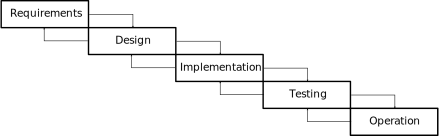
\includegraphics[width=\textwidth]{assets/sdlc.pdf}
	\caption{Improved Waterfall model by Royce}
	\label{fig:waterfall-royce}
\end{figure}

\noindent In this thesis I will solely focus on the implementation and testing phase, as these are the most time-consuming phases of the entire process. The modification to the Waterfall model by Royce is particularly useful when applied to these two phases, in the context of \emph{software regressions}. A regression \cite{10.1007/978-3-540-77966-7_18} is a feature that was previously working correctly, but is now malfunctioning. This behaviour can have external causes, such as a change in the system clock because of daylight saving time, but can also be the result of a change to another, seemingly unrelated part of the application code \cite{6588537}.\\

\noindent Software regressions and other functional bugs can ultimately incur disastrous effects, such as severe financial loss or damage to the reputation of the software company. The most famous example in history is without any doubt the explosion of the Ariane 5-rocket, which was caused by an integer overflow \cite{581900}. In order to reduce the risk of bugs, malfunctioning components should be detected as soon as possible to proactively defend against potential failures. Because of this reason, the testing phase is to be considered as the most important phase of the entire development process and an application should therefore include sufficient tests. The collection of all tests included in an application, or a smaller chosen subset of certain tests, is referred to as the \emph{test suite}. Tests can be classified in multiple categories, this thesis will consider three distinguishable categories:

\begin{enumerate}
	\bolditem{Unit test} This is the most basic kind of test. The purpose of a unit test is to verify the behaviour of an individual component \cite{whittaker2000}. The scope of a unit test should be limited to a small and isolated piece of code, such as one function. Unit tests are typically implemented as \emph{white-box tests} \cite[p.~12]{6588537}. A white-box test is constructed by manually inspecting the function under test, to identify important \emph{edge values}. The unit test should then feed these values as arguments to the function under test, to observe its behaviour. Common edge cases include zero, negative numbers, empty arrays or array boundaries that might result in an overflow.
	
	\bolditem{Integration test} A more advanced test, an integration test verifies the interaction between multiple individually tested components \cite{whittaker2000}. Examples of integration tests include the communication between the front-end and the back-end side of an application. As opposed to unit tests, an integration test is an example of a \emph{black-box} test \cite[p.~6]{6588537}, meaning that implementation-specific details should be irrelevant or unknown when writing an integration test.
	
	\bolditem{Regression test} After a regression has been detected, a regression test \cite[p.~372]{8016712} is added to the test suite. This regression test should replicate the exact conditions and sequence of actions that have caused the regression, to warden the implementation against subsequent failures if the same conditions would reapply in the future.
\end{enumerate}

% !TeX root = ../../thesis.tex

\subsection{Test Suite Assessment}

\subsubsection{Coverage}
\noindent The most frequently used metric to measure the quantity and thoroughness of a test suite is the \emph{code coverage} or \emph{test coverage} \cite[p.~467]{8016712}. The test coverage is expressed as a percentage and indicates which fraction of the application code is affected by code in the test suite. Internally, this works by augmenting every statement in the application code using binary instrumentation. A hook is inserted before and after every statement to keep track of which statements are executed during tests. Many different criteria exist to interpret these instrumentation results and thus to express the fraction of covered code \cite{Myers:2011:AST:2161638}, the most commonly used ones are \emph{statement coverage} and \emph{branch coverage}.

\paragraph*{Statement coverage} expresses the fraction of code statements that are executed in any test of the test suite \cite{6588537}, out of all executable statements in the application code. Analogously, the fraction of lines covered by a test may be used to calculate the \emph{line coverage} percentage. Since one statement can span multiple lines and one line may also contain more than one statement, both of these criteria implicitly represent the same value. Statement coverage is heavily criticised in literature \cite[p.~37]{Myers:2011:AST:2161638}, since it is possible to achieve a statement coverage percentage of 100\% on a code fragment which can be proven to be incorrect. Consider the code fragment in \autoref{lst:statement-coverage-fail}. If a test would call the \texttt{example}-function with arguments $\{a = 1, b = 2\}$, the test will pass and every statement will be covered, resulting in a statement coverage of 100\%. However, it is clear to see that if the function would be called with arguments $\{a = 0, b = 0\}$, a \emph{division-by-zero} error would be raised, resulting in a crash. This very short example already indicates that statement coverage is not trustworthy, yet it may still be useful for other purposes, such as detecting unreachable code which may safely be removed.

\begin{listing}
	\begin{lstlisting}[language=C]
		int example(int a, int b) {
			if (a == 0 || b != 0) {
				return a / b;
			}
		}
	\end{lstlisting}
	\captionsetup{skip=-2pt}
	\caption{Example of irrelevant statement coverage in C.}
	\label{lst:statement-coverage-fail}
\end{listing}

\paragraph*{Branch coverage} on the other hand, requires that every branch of a conditional statement is traversed at least once \cite[p.~37]{Myers:2011:AST:2161638}. For an \texttt{if}-statement, this results in two tests being required, one for every possible outcome of the condition (\texttt{true} or \texttt{false}). For a \texttt{loop}-statement, this requires a test case in which the loop body is never executed and another test case in which the loop body is always executed. Remark that while this criterion is stronger than statement coverage, it is still not sufficiently strong to detect the bug in \autoref{lst:statement-coverage-fail}. In order to mitigate this, \emph{multiple-condition coverage} \cite[p.~40]{Myers:2011:AST:2161638} is used. This criterion requires that for every conditional statement, every possible combination of subexpressions is evaluated at least once. Applied to \autoref{lst:statement-coverage-fail}, the \texttt{if}-statement is only covered if the following four cases are tested, which is sufficient to detect the bug.
\begin{itemize}
	\item $a = 0, b = 0$
	\item $a = 0, b \neq 0$
	\item $a \neq 0, b = 0$
	\item $a \neq 0, b \neq 0$
\end{itemize}

\noindent It should be self-evident that achieving and maintaining a coverage percentage of 100\% at all times is critical. However, this does not necessarily imply that all lines, statements or branches need to be covered explicitly \cite{dein_2019}. Some parts of the code might simply be irrelevant or untestable. Examples include wrapper or delegation methods that simply call a library function. All major programming languages have frameworks and libraries available to collect coverage information during test execution, and each of these frameworks allows the developer to exclude parts of the code from the final coverage calculation. As of today, the most popular options are JaCoCo\footnote{\url{https://www.jacoco.org/jacoco/}} for Java, coverage.py\footnote{\url{https://github.com/nedbat/coveragepy}} for Python and simplecov\footnote{\url{https://github.com/colszowka/simplecov}} for Ruby. These frameworks are able to generate in-depth statistics on which parts of the code are covered and which parts require more tests, as illustrated in \autoref{fig:coverage-statistics}.

\subsubsection{Mutation testing}
Whereas code coverage can be used to identify whether or not a part of the code is currently affected by the test suite, \emph{mutation testing} can be used to measure its quality and ability to detect future failures. This technique creates several syntactically different instances of the source code, referred to as \emph{mutants}. A mutant can be created by applying one or more \emph{mutation operators} to the original source code. These mutation operators are aimed at simulating typical mistakes that developers tend to make, such as the introduction of off-by-one errors, removal of statements and replacement of logical connectors \cite{Offutt2001}. The \emph{mutation order} refers to the amount of mutation operators that have been applied consecutively to an instance of the code. This order is traditionally rather low, as a result of the \emph{Competent Programmer Hypothesis}, which states that programmers develop programs which are near-correct \cite{5487526}.

\paragraph*{Creating and evaluating} the mutant versions of the code is a computationally expensive process and requires human intervention, which is why very few software developers have managed to employ this technique in practice. \autoref{fig:mutation-testing} shows how mutation testing is performed. First of all, the mutation system takes the original program $P$ and a set of test cases $T$. Then, several mutation operators are applied to construct a large set of mutants $P'$. The next step is to evaluate every test case $t$ on the original program $P$ to verify its correctness, this is a task that needs to be performed manually. If at least one of these test cases proves incorrect, a bug has been found in the original program, which needs to be resolved before the mutation analysis can continue. When $P$ successfully passes every test case, every test case are evaluated for each of the mutants. A mutant $p'$ is said to be ``killed'' if its output is different from $P$ for at least one test case, otherwise it is considered ``surviving''. After executing all test cases, the set of surviving mutants should be analysed in order to introduce subsequent test cases that can be used to kill them. However, it is also possible that the surviving mutants are functionally equivalent to $P$. This needs to be verified manually, since the detection of program equivalence is impossible \cite{5487526, Offutt2001}.

\begin{figure}[htbp!]
	\centering
	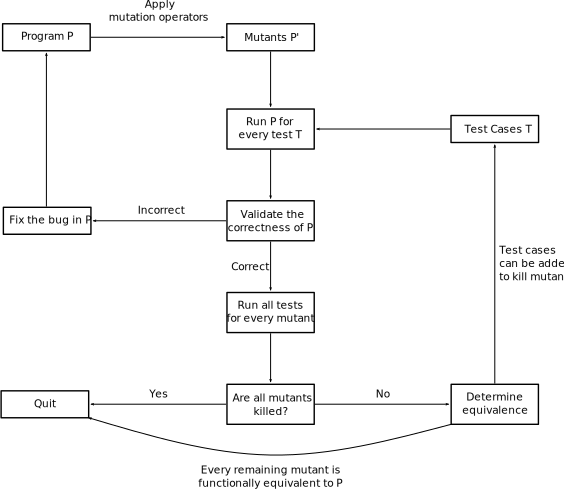
\includegraphics[width=\textwidth]{assets/mutation-testing.pdf}
	\caption{Process of Mutation Testing (based on \cite{Offutt2001})}
	\label{fig:mutation-testing}
\end{figure}

\noindent After every mutant has either been killed or marked equivalent to the original problem, a \emph{mutation score} is calculated using \autoref{eq:mutant-score}. In a perfect test suite, this score should be equal to 1, indicating that the test suite was able to detect every mutant. 

\begin{equation}\label{eq:mutant-score}
	\text{Mutant Score} = \frac{\text{killed mutants}}{\text{non-equivalent mutants}}
\end{equation}


\begin{figure}[htbp!]
	\centering
	\subfloat[JaCoCo coverage report of \url{https://github.com/thepieterdc/dodona-api-java}]{%
		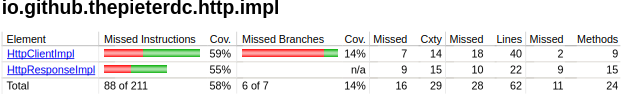
\includegraphics[clip,width=\textwidth]{assets/coverage-jacoco.pdf}
	}
	\newline
	\subfloat[coverage.py report of \url{https://github.com/codecov/example-python}]{%
		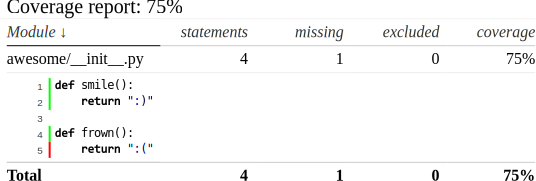
\includegraphics[clip,width=\textwidth]{assets/coverage-coveragepy.pdf}
	}
	\newline
	\subfloat[simplecov report of \url{https://github.com/dodona-edu/dodona}]{%
		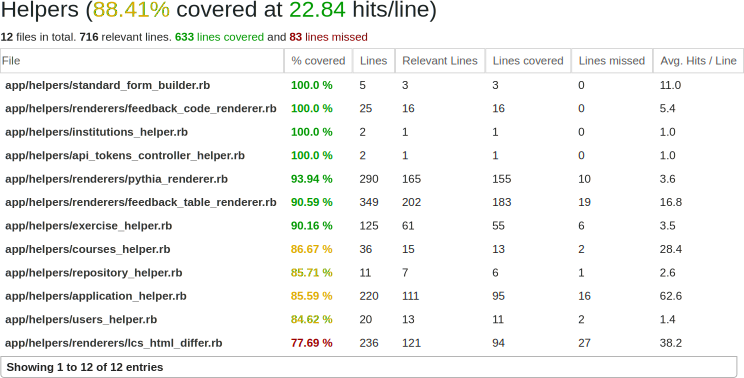
\includegraphics[clip,width=\textwidth]{assets/coverage-simplecov.pdf}
	}
	\caption{Statistics from Code coverage tools}
	\label{fig:coverage-statistics}
\end{figure}
\newpage
% !TeX root = ../thesis.tex

\section{Agile Software Development}
% !TeX root = ../../thesis.tex

\subsection{Agile Manifesto}
Since the late 1990s, developers have tried to reduce the time occupied by the implementation and testing phases. As a result, several software pioneers have proposed new implementations of the SDLC, which were later collectively referred to as the \emph{Agile development methodologies}. This term was coined during a meeting of seventeen prominent software developers, in which they have defined the following four fundamental values of Agile development in the \emph{Agile Manifesto} \cite{beck2001agile}.

\begin{enumerate}
	\item \emph{Individuals and interactions} over processes and tools.
	\item \emph{Working software} over comprehensive documentation.
	\item \emph{Customer collaboration} over contract negotiation.
	\item \emph{Responding to change} over following a plan.
\end{enumerate}

\noindent According to the authors, we should interpret these values as follows: ``While there is value in the items on the right, we value the items on the left more'' \cite{beck2001agile}. When we examine these values more closely, we can observe that they all share a common philosophy, which is that software engineering should be a fast process in which communication and a short feedback loop is critical to avoid missteps. Since 2001, a variety of different programming models have arisen, each incorporating these Agile principles in their own way. The most remarkable new practice is \acrfull{tdd}. Recall that an integration test is a black-box test and that as such, we can actually construct the test case in advance and write the implementation afterwards. This concept is also prevalent in TDD. This practice depicts that if we want to extend the functionality of the application, we should first modify the test cases (or add new test cases) and then modify the application code until every test case is passing \cite{10.5555/579193}.
% !TeX root = ../../thesis.tex

\subsection{The need for Agile}
In the wake of the world economic crisis, software companies were forced to devote efforts into researching how their overall expenses could be reduced. This research has concluded that in order to reduce financial risks, the \emph{time-to-market} of an application should be as short as possible. In order to accomplish this, further research was conducted, resulting in an increase of attention for agile methodologies in scientific literature \cite{ionel2009}. As was previously described in \autoref{sssec:agilevalue-workingsoftware}, agile methodologies strive to deliver a minimal version as soon as possible, allowing additional functionality to be added in an incremental fashion. This effectively results in a shorter \emph{time-to-market} and lower costs, since the company can decide to cancel the project much earlier in the process.\\

\noindent In addition to a reduced time-to-market, maintaining an agile workflow has also proven beneficial to the success rate of development. A study performed by The Standish Group revealed that the success rate of agile projects is more than three times higher compared to when traditional methodologies are practised \cite[p.~7]{standish2015chaos}, as illustrated in \autoref{fig:agile-success-rate}. 

\begin{figure}[htbp!]
	\centering
	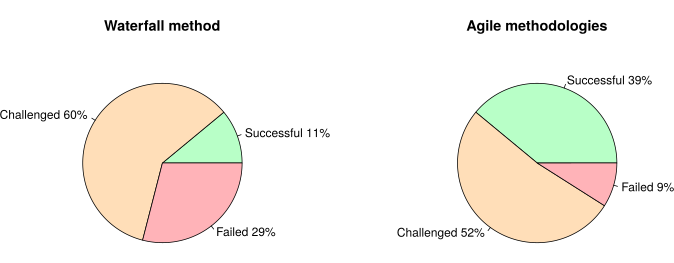
\includegraphics[width=\textwidth]{assets/agile-success-rate.pdf}
	\caption{Success rate of Agile methodologies \cite{standish2015chaos}.}
	\label{fig:agile-success-rate}
\end{figure}



%hier in hoofdstuk 7 staat iets over continuous integration
%https://link.springer.com/chapter/10.1007/978-3-319-05155-0_7

- changes moeten zeer regelmatig worden geintegreerd met elkaar -> feedback loop tussen implement -> integrate -> test -> repeat
- Continuous integration: wat?
- Bestaan aantal bestaande frameworks voor
- Maar; dat testen kan heel lang duren (zoek een bron waarin lange tests besproken worden)
- Bestaan aantal oplossingen voor -> zie volgende hoofdstuk

- feedback loop

- buildup naar waarom tooling nodig is

- waarom

- wat

- voorbeelden: Jenkins, CircleCI, Travis-CI, recent GitHub Actions + screenshots

- Probleem en oplossingen met regression tests


\section{Continuous Integration}
\subsection{Agile Manifesto}
Since the late 1990's, developers have tried to reduce the time occupied by the implementation and testing phases. In order to accomplish this, several new implementations of the SDLC were proposed and evaluated, later collectively referred to as \emph{Agile development methodologies}. The term \emph{Agile development} was coined during a meeting of seventeen prominent software developers, held between February 11-13, 2001, in Snowbird, Utah \cite{jimhighsmith2001}. As a result of this meeting, the developers defined the four key values and twelve principles that define these new methodologies, called the \emph{Manifesto for Agile Software Development}, also known as the \emph{Agile Manifesto}.

\subsubsection{Four values}

The four key values of Agile programming should be interpreted as follows, according to the authors: "While there is value in the items on the right, we value the items on the left more" \cite{beck2001agile}. It should be noted that these values are merely guidelines and that no concrete implementation is provided. A variety of different programming models have arisen since 2001, each incorporating these values in their own unique way.

// TODO ZIE hazzan2014 paper

\begin{enumerate}
	\item \textbf{\emph{Individuals and interactions} over processes and tools:} (TODO explain)
	\item \textbf{\emph{Working software} over comprehensive documentation:} (TODO explain)
	\item \textbf{\emph{Customer collaboration} over contract negotiation:} (TODO explain)
	\item \textbf{\emph{Responding to change} over following a plan:} (TODO explain)
\end{enumerate}

\subsubsection{Twelve principles}
\begin{enumerate}
	\item \textbf{(TODO principle 1)} (TODO explain)
	\item \textbf{(TODO principle 2)} (TODO explain)
	\item \textbf{(TODO principle 3)} (TODO explain)
	\item \textbf{(TODO principle 4)} (TODO explain)
	\item \textbf{(TODO principle 5)} (TODO explain)
	\item \textbf{(TODO principle 6)} (TODO explain)
	\item \textbf{(TODO principle 7)} (TODO explain)
	\item \textbf{(TODO principle 8)} (TODO explain)
	\item \textbf{(TODO principle 9)} (TODO explain)
	\item \textbf{(TODO principle 10)} (TODO explain)
	\item \textbf{(TODO principle 11)} (TODO explain)
	\item \textbf{(TODO principle 12)} (TODO explain)
\end{enumerate}

\subsection{The need for Agile}
Over the past decade, the agile methodologies have received increasing attention amongst software developers, following the world economic crisis of 2009 \cite{ionel2009}. A consequence of this crisis was that software companies were forced to cut on their expenses and find ways to reduce the \emph{time-to-market} of their applications.

- probleem met waterfall model -> een bron hiervoor?

- feedback loop

- buildup naar waarom tooling nodig is

- waarom

- wat

- voorbeelden: Jenkins, CircleCI, Travis-CI, recent GitHub Actions + screenshots

- Probleem en oplossingen met regression tests

  - Test Case Prioritization -> Focus want geen tests weggooien
  
  - Test Suite Minimization
  
  - Test Suite Selection
  
  - Test Suite Reduction


\clearpage
%% !TeX root = thesis.tex

WIJ-ificeren!!!!!!!!!!!!!!!!!!!!!

\chapter{Related work}
\label{ch:related-work}
The previous chapter has stressed the paramount importance of frequently integrating one's changes into the upstream repository. This process can be a complex and lengthy operation. As a result, software engineers have sought and found ways to automate this task. These solutions and practices embody \acrfull{ci}. However, \acrshort{ci} is not the golden bullet for software engineering, as there is a flip side to applying this practice. After every integration, the entire test suite must be executed to ensure that no regression has been introduced. As the project evolves and the size of the codebase increases, the number of test cases will increase accordingly to preserve a sufficiently high coverage level \cite{evaluationoftestsuiteminimization}. Walcott, Soffa and Kapfhammer illustrate the magnitude of this problem by providing an example of a project consisting of \SI{20000}{} lines of code. The test suite of this project requires up to seven weeks to complete \cite{10.1145/1146238.1146240}.\\

TODO DEZE PARAGRAAF
\noindent Fortunately, multiple developers and researchers have found some techniques that can be used to address the scalability issues of growing test suites. The techniques currently known to literature can be classified in three categories. Developers can either apply \emph{\tsm{}}, \emph{\tcs{}} or \emph{\tcp{}} \cite{evaluationoftestsuiteminimization}. All three techniques are applicable to any test suite, however there is a trade-off to be made. Depending on which technique is chosen, it will either have a major impact on the duration of the test suite execution in exchange for a reduced test coverage level, or it will result in a higher test adequacy.\\

\noindent The following sections will discuss these three approaches in more detail and provide accompanying algorithms. Because the techniques are very similar, the corresponding algorithms can (albeit with minor modifications) be used interchangeably for every approach. The final section of this chapter will investigate the adoption and integration of these techniques in modern software testing frameworks.

% !TeX root = ../thesis.tex

\section{Classification of approaches}

% !TeX root = ../../thesis.tex

\subsection{\tsm{}}
\label{ssec:tsm}
The first technique is called \acrfull{tsm}, also referred to as \emph{Test Suite Reduction} in literature. This technique will try to reduce the size of the test suite by permanently removing redundant test cases. This problem has been formally defined by Rothermel \cite{10.1002/stv.430} in \cref{def:tsm} and illustrated in \Cref{fig:tsm}.

\begin{definition}[\tsm{}]
\label{def:tsm}
\mbox{}\\Given:
\begin{itemize}
	\item $T = \{t_1, \dots, t_n\}$ a test suite consisting of test cases $t_j$.
	\item $R = \{r_1, \dots, r_m\}$ a set of requirements that must be satisfied in order to provide the desired ``adequate'' testing of the program.
	\item $\{T_1, \dots, T_m\}$ subsets of test cases in $T$, one associated with each of the requirements $r_i$, such that any one of the test cases $t_j \in T_i$ can be used to satisfy requirement $r_i$.
\end{itemize}

\noindent Subsequently, we can define \tsm{} as the task of finding a subset $T'$ of test cases $t_j \in T$ that satisfies every requirement $r_i$.
\end{definition}

\noindent If we apply the concepts of the previous chapter to the above definition, we can interpret the set of requirements $R$ as source code lines that must be covered. A requirement $r_i$ can subsequently be satisfied by any test case $t_j \in T$ that belongs to the subset $T_i$. Observe that the problem of finding $T'$ is closely related to the \emph{hitting set problem} (\cref{def:hitting-set}) \cite{10.1002/stv.430}.

\begin{definition}[Hitting Set Problem]
\label{def:hitting-set}
\mbox{}\\Given:
\begin{itemize}
	\item $S = \{s_1, \dots, s_n\}$ a finite set of elements.
	\item $C = \{c_1, \dots, c_n\}$ a collection of sets, with $\forall c_i \in C : c_i \subseteq S$.
	\item $K$ a positive integer, $K \le |S|$.
\end{itemize}

\noindent The hitting set is a subset $S' \subseteq S$ such that $S'$ contains at least one element from each subset in $C$.
\end{definition}

\noindent In the context of \tsm{}, $T'$ corresponds to the hitting set of $T_i$s. In order to effectively minimise the amount of tests in the test suite, $T'$ should be the minimal hitting set \cite{10.1002/stv.430}. Since we can reduce this problem to the NP-complete \emph{Vertex Cover}-problem, we know that this problem is NP-complete as well \cite{10.5555/574848}.

\begin{figure}[htbp!]
	\centering
	\includegraphics[width=\textwidth]{assets/tikz/approach-tsm.tikz}
	\caption{\tsm{}}
	\label{fig:tsm}
\end{figure}
% !TeX root = ../../thesis.tex

\subsection{\tcs{}}
The second algorithm closely resembles the previous one. Instead of determining the minimal hitting set of the test suite in order to permanently remove tests, this algorithm has a notion of context. Prior to the execution of the tests, the algorithm performs a \emph{white-box static analysis} of the codebase to identify which parts have been changed. Subsequently, only the tests regarding modified parts are executed, making the selection temporary (\autoref{fig:tcs}) and modification-aware \cite{10.1002/stv.430}. Rothermel and Harrold define this formally in \autoref{def:tcs}.

\begin{definition}[\tcs{}]
\label{def:tcs}
\mbox{}\\Given:
\begin{itemize}
	\item $P$ the previous version of the codebase
	\item $P'$ the current (modified) version of the codebase
	\item $T$ the test suite
\end{itemize}

\noindent \tcs{} aims to find a subset $T' \subseteq T$ that is used to test $P'$. 
\end{definition}

\begin{figure}[htbp!]
	\centering
	
\includegraphics[width=0.45\textwidth]{assets/placeholder.pdf}
	\caption{\tcs{}}
	\label{fig:tcs}
\end{figure}
% !TeX root = ../../thesis.tex

\subsection{\tcp{}}
Both \acrshort{tsm} and \acrshort{tcs} attempt to execute as few tests as possible to reduce the execution time of the test suite. Nevertheless, in some cases, we may require to execute every test case to guarantee correctness. In this situation, we can still optimise the test suite. \acrfull{tcp} aims to find a permutation of the sequence of test cases, rather than eliminating specific tests from being executed (\Cref{fig:tcp}). We choose the order of the permutation in such a way that we can complete a predefined objective as soon as possible. Once we have achieved our objective, we can early terminate the execution of the test suite. In the worst-case scenario, we will still execute every test case. Some examples of objectives include covering as many lines of code as fast as possible or executing tests ordered on their probability of failure \cite{10.1002/stv.430}. \Cref{def:tcp} provides a formal definition of this approach.

\begin{definition}[\tcp{}]
\label{def:tcp}
\mbox{}\\Given:
\begin{itemize}
	\item $T$ the test suite
	\item $PT$ the set of permutations of $T$
	\item $f: PT \mapsto \mathbb{R}$ a function from a subset to a real number, this function is used to compare sequences of test cases to find the optimal permutation.
\end{itemize}

\noindent \tcp{} finds a permutation $T' \in PT$ such that $\forall T'' \in PT : f(T') \ge f(T'') \Rightarrow (T'' \ne T')$ 
\end{definition}

\begin{figure}[htbp!]
	\centering
	\includegraphics[width=\textwidth]{assets/tikz/approach-tcp.tikz}
	\caption{\tcp{}}
	\label{fig:tcp}
\end{figure}
\newpage
\section{Algorithms}
\noindent This thesis prefers to use TCP since this technique does not incur the risk of false-negative failing test cases. In order to determine the optimal order of execution, this thesis presents three existing algorithms.\\

\noindent The input data for these algorithms is threefold:\\

\begin{itemize}
\item \textbf{Affected test cases:} By combining previous coverage results and the list of changes that the developer has made to the code, the framework can estimate which test cases are likely affected by those changes and assign a higher priority.

\item \textbf{Historical data:} Next, historical failure data can be used. Suppose that a test case has failed in its previous execution, then there exists a chance that it will subsequently fail in the current run.

\item \textbf{Execution timings:} Finally, if two test cases are considered equally likely to fail, the average duration of the test case can be used as a tie-breaker. Since the objective of TCP is to optimise the test suite, the test case with the lowest duration should be preferred.
\end{itemize}

\subsection{Greedy algorithm}
\noindent The first algorithm is a greedy heuristic that was initially designed as an algorithm for the set-covering problem \cite{evaluationoftestsuiteminimization}. This heuristic starts with an empty set of test cases and the set of all code lines $C$. Next, the algorithm iteratively selects the test case that contributes the most code lines that are not yet covered, updating $C$ after every selected test case. The algorithm halts when either all test cases are selected or $C$ is empty. In order to modify this algorithm to make it applicable to TCP, the selection order must be preserved and used as the prioritised sequence.

\subsection{HGS algorithm}
\noindent The second algorithm was created by Harrold, Gupta and Soffa \cite{hgs}. As opposed to the greedy heuristic, this algorithm uses a different perspective. First, the algorithm sorts the code lines increasingly based on the number of test cases that cover them. The motivation for this sorting operation is that some test cases must inevitably be executed, as they are the only test cases that cover a given set of lines. However, these test cases can also cover other lines and therefore make other test cases redundant. The algorithm iterates over the code lines in this order and selects one corresponding test case in each iteration. Afterwards, the order is updated to remove source code lines which are now covered by the selected test case. This process is repeated until there are no lines left to cover.

\clearpage

\subsection{ROCKET algorithm}
\noindent Finally, this thesis considers the ROCKET algorithm \cite{6676952}. This algorithm prioritises test cases by assigning a score to every test case, which is calculated using historical failure data. Afterwards, the algorithm computes the cumulative score $CS_t$ of every test case $t$ and defines the following objective function $g$, in which $E_t$ represents the execution time of the test case:
$$g = (maximise(CS_t), minimise(E_t))$$

\noindent Finally, the algorithm optimises this function to determine the ideal order of execution $S$, as follows:
$$(\forall i \in 1 \dots n)(g(S_i) \ge g(S_{i+1})$$
\newpage
% !TeX root = ../thesis.tex

\section{Adoption in testing frameworks}
In the final section of this chapter, we will investigate how existing software testing frameworks have implemented these and other optimisation techniques.

% !TeX root = ../../thesis.tex

\subsection{Gradle and JUnit}\label{ssec:relatedwork-gradle-junit}
Gradle\footnote{\url{https://gradle.org}} is a dependency manager and application framework for Java, Groovy and Kotlin projects. Gradle supports multiple plugins to automate tedious tasks, such as configuration management, testing and deploying. One of the supported testing integrations is \junit{\footnote{\url{https://junit.org}}, which is the most widely used unit testing framework by Java developers. \junit{} 5 is the newest version which is still actively being developed as of today. The framework is integrated as the testing framework of choice in several other Java libraries and frameworks, such as Android and Spring. \junit{} offers mediocre support for features that optimise the execution of the test cases, especially when used in conjunction with Gradle. The following three key features are available:
\begin{enumerate}
	\item \textbf{Parallel test execution:} JUnit comes bundled with multiple test processors that are responsible for processing test classes and to execute the test cases. One of these test processors is the \texttt{MaxNParallelTestClassProcessor}, which is capable of running a configurable amount of test cases in parallel. This results in a major speed-up of the overall test suite execution.

	\item \textbf{Prioritise failed test cases:} Another test class processor which is provided by Gradle, is the \texttt{RunPreviousFailedFirstTestClassProcessor}. This processor will prioritise test cases that have failed in the previous run, similar to the idea of the ROCKET-algorithm (\autoref{ssec:alg-rocket}), albeit without taking into account the duration of these test cases.
	
	\item \textbf{Test order specification:} JUnit allows the user to specify the order in which test cases will be executed\footnote{\url{https://junit.org/junit5/docs/current/user-guide/\#writing-tests-test-execution-order}}. By default, a random yet deterministic order is used. The order can be manipulated by annotating the test class with the \texttt{@TestMethodOrder}-annotation, or by annotating individual test cases with the \texttt{@Order(int)}-annotation. This feature can only be used to alter the order of test cases within the same test class, it is not possible to perform inter-test class reordering. This feature could be used to sort test cases based on their execution time.
\end{enumerate}

\begin{figure}[htbp!]
	\centering
	\begin{minipage}{.45\textwidth}
		\centering
		
\includegraphics[width=0.8\textwidth]{assets/gradle.pdf}
		\caption{Logo of Gradle}
	\end{minipage}
	\begin{minipage}{.45\textwidth}
		\centering
		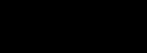
\includegraphics[width=0.6\textwidth]{assets/junit.pdf}
		\caption{Logo of JUnit 5}
	\end{minipage}
\end{figure}
% !TeX root = ../../thesis.tex

\subsection{Maven Surefire}
A commonly used alternative to Gradle is Apache Maven\footnote{\url{http://maven.apache.org/}}. This framework also supports executing JUnit test cases using the Surefire plugin. As opposed to Gradle, Surefire does offer multiple options to specify the order in which the test cases will be executed using the \texttt{runOrder} property. Without any configuration, Maven will run the test cases in alphabetical order. By switching the \texttt{runOrder} property to \texttt{failedFirst}, we can tell Maven to prioritise the previously failed test cases. Another supported value is \texttt{balanced}, which orders test cases based on their duration. Finally, we can choose to implement a custom ordering scheme for absolute control.
% !TeX root = ../../thesis.tex

\subsection{OpenClover}
OpenClover\footnote{\url{https://openclover.org}} is a code coverage tool for Java and Groovy projects. It was created by Atlassian and open-sourced in 2017. OpenClover profiles itself as ``the most sophisticated code coverage tool'', by extracting useful metrics from the coverage results and by providing features that can optimise the test suite. These features include powerful integrations with development software and prominent Continuous Integration systems. Furthermore, OpenClover can automatically analyse the coverage results to detect relations between the application source code and the test cases. This feature allows OpenClover to predict which test cases will have been affected, given a set of modifications to the source code. Subsequently, we can interpret these predictions to implement \tcs{} and therefore reduce the test suite execution time.
\clearpage
%% !TeX root = thesis.tex

\chapter{Proposed framework: \velocity{}}
\clearpage
%% !TeX root = thesis.tex

\chapter{Evaluation}
\label{ch:evaluation}
This chapter will evaluate the performance of framework presented in the previous chapter. In the first section, the two test subjects that will be used in the subsequent experiments will be introduced. The next section will restate the research questions formally, and extend these. Afterwards, the procedure of how the data was obtained will be elaborated. The final section will provide answers to the research questions as well as present the results of applying \tcp{} to the test subjects.

% !TeX root = ../thesis.tex

\section{Test subjects}

\subsection{Dodona}
Dodona\footnote{\url{https://dodona.ugent.be/}} is an open source online learning environment created by Ghent University, allowing students from secondary schools and universities in Belgium and South-Korea to submit solutions to programming exercises and receive automated feedback. The application is built using the Ruby-on-Rails web framework. In order to automate the testing process of the application, Dodona makes use of Github Actions (\autoref{sssec:github-actions}) to run tests using the default \texttt{MiniTest} testing framework. The coverage of the test suite is being recorded by \texttt{SimpleCov}\footnote{\url{https://github.com/colszowka/simplecov}}.

\subsection{Stratego}
Leg uit wat het is.
% !TeX root = ../thesis.tex

\section{Research questions}
We will answer the following research questions in the subsequent sections:

\paragraph*{RQ1: What is the probability that a test run will contain at least one failed test case?}
The first research question will provide useful insights into whether a typical test run tends to fail or not. The expectancy is that the probability of failure will be rather low, indicating that it is not strictly necessary to execute every test case and therefore making a case for \tsm{}.

\paragraph*{RQ2: What is the average duration of a test run?}
Measuring how long it takes to execute a typical test run is required to estimate the benefit of applying any form of test suite optimisation. We will only consider successful test runs, to reduce bias introduced by prematurely aborting the execution.

\paragraph*{RQ3: Suppose that a test run has failed, what is the probability that the next run will fail as well?}
The ROCKET algorithm (\cref{ssec:alg-rocket}) relies on the assumption that if a test case has failed in a given test run, it is likely to fail in the subsequent run as well. This research question will investigate the correctness of this hypothesis.

\paragraph*{RQ4: How can \tcp{} be applied to Dodona and what is the resulting performance benefit?}
This research question will investigate the possibility to apply the \velocity{} framework to the Dodona project and analyse how quickly the available predictors can discover a failing test case.

\paragraph*{RQ5: Can the Java agent be applied to Stratego?}
Since the testing framework used by Stratego should be supported natively by the Java agent, this research question will verify its compatibility. Furthermore, we will analyse the prediction performance, albeit with a small number of relevant test runs.
% !TeX root = ../thesis.tex

\section{Data collection}\label{sec:eval-data}

\subsection{\travisci{} build data}
In order to answer the first three research questions, build data for several projects hosted on \travisci{} (\autoref{sssec:travisci}) was used. This data was obtained from two sources.\\

\noindent The first source is a database of \SI{35793144} jobs, provided by Durieux et al \cite{travisanalysis}. Due to the magnitude of this dataset (\SI{61.11}{\gibi\byte}), a big data framework is required to parse the log files. In order to collect the required data for the three first research questions, three MapReduce pipelines have been created using the Apache Spark\footnote{\url{https://spark.apache.org/}} framework.\\



\noindent Additionally, another \SI{3702595} jobs have been analysed from the \emph{TravisTorrent} project. This project \cite{msr17challenge} scrapes the API of \travisci{} and combines this with data obtained from the GitHub API to infer additional information about the test run, such as the programming language and the amount of failed test cases. The creators of TravisTorrent have provided a Google BigQuery\footnote{\url{https://bigquery.cloud.google.com/}} interface to allow querying the dataset. The following queries have been executed:

\subsection{Dodona build data}
// bespreek dodona instrumenter.
\clearpage
% !TeX root = ../thesis.tex

\section{Results}

\subsection{RQ1: Probability of failure}\label{ssec:results-rq1}
\autoref{fig:rq1-failure-probability} contains two pie charts that illustrate the amount of failed and successful test runs. The left chart contains the results of the dataset provided by Durieux et al \cite{travisanalysis}. This dataset contains $\SI{4558279}{}$ failed test runs versus $\SI{24323724}{}$ successful runs, which corresponds to a failure probability of $\SI{18.74}{\percent}$. The other pie chart visualises data from the TravisTorrent project. According to this dataset, the run has failed prior to starting the test suite in $\SI{42.89}{\percent}$ of the executions. For the remaining part of the runs, $\SI{225766}{}$ out of $\SI{2114920}{}$ executions contained at least one failed test case, corresponding to a failure percentage of $\SI{10.67}{\percent}$.

\begin{figure}[htbp!]
	\centering
	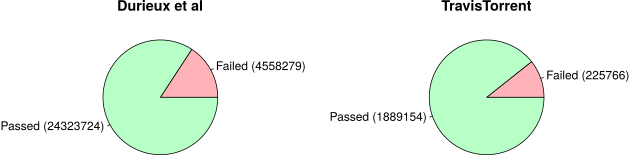
\includegraphics[width=\textwidth]{assets/charts/rq1-failure-probability.pdf}
	\caption{Probability of test run failure}
	\label{fig:rq1-failure-probability}
\end{figure}

\subsection{RQ2: Probability of consecutive failure}
In order to find consecutive failures, only the TravisTorrent project can be used as every entry in this dataset contains the identifier of the previous build which is required to link consecutive builds. The dataset contains $\SI{211040}{}$ test runs of which the test suite of the preceding test run was both executed and contained at least one failed test case. As illustrated in \autoref{fig:rq2-consecutive-failure}, $\SI{109224}{}$ of these test runs failed as well, versus $\SI{101816}{}$ test runs ($\SI{51.76}{\percent}$) that did succeed.

\begin{figure}[htbp!]
	\centering
	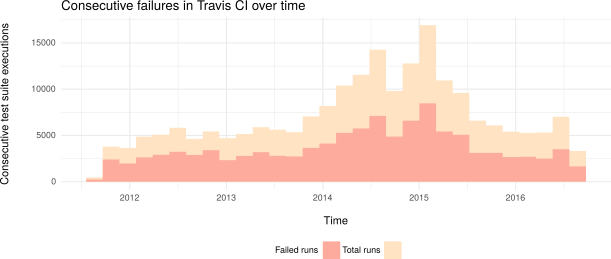
\includegraphics[width=\textwidth]{assets/charts/rq2-consecutive-failure.pdf}
	\caption{Consecutive test run failures on \travisci{}}
	\label{fig:rq2-consecutive-failure}
\end{figure}

\subsection{RQ3: Average test run duration}

maak boxplot van 5.3

- tests lager dan 10 seconden werden genegeerd aangezien dit een failure in de setup betekent.
- de zeer lange tests maken gebruik van mutation testing
- gegroepeerd per hoeveelheid en genormaliseerd op de y-as


\subsection{RQ4: Applying \tcp{} to Dodona}

voor 5.4:

- duration per run
- failed test cases per run
- time (ms) until first failed test case
- time (ms) until first prioritised failed test case
\clearpage
%% !TeX root = thesis.tex

\chapter{Conclusion}
\label{ch:conclusion}

The main purpose of this thesis has been to investigate different approaches towards optimising the test suite of a common software project. The concepts of \tsm{}, \tcs{} and \tcp{} have been introduced and accompanying algorithms have been presented. A novel client-server oriented framework for the latter approach has been proposed, as well as a new prioritisation algorithm. Finally, \velocity{} has been applied to the UGent Dodona project, proving its ability to predict test case failure and therefore reduce the execution time of the test suite.\\

\noindent A second purpose of this thesis was to gain useful insights into the behaviour of a typical test suite. These insights have been formulated as three additional research questions, to which answers have been provided in the previous chapter.

\section{Future work}
The proposed \velocity{} implementation in this thesis is currently able to prioritise a Gradle Java project using 10 available predictors and a meta predictor. While this is certainly functional, it is far from complete and multiple improvements can be added.

\subsection{Java Agent}
The existing Java Agent can be extended in multiple ways. The most prominent addition would be to allow test cases to be executed in parallel. At the moment of writing, this is not possible yet. In order to facilitate parallel testing, one must first decide how to schedule the prioritised test cases across multiple threads, since the execution time of a test case varies strongly. One possibility to perform this scheduling is to use the average execution time per test case, which is obtained from prior runs. Alternatively, this can be performed at runtime by using any existing inter-thread communication paradigm such as message passing. On the implementation side of parallelisation, the current \texttt{TestProcessor} should be adapted to inherit from the \texttt{MaxNParallelTestClassProcessor}. A thread pool should ideally be used to reduce the overhead of restarting a new thread for every test case.

\subsection{Predictions}
Further research and improvements to the predictors can be made on four different aspects.\\

\noindent The first enhancement is that currently the predictor does not discriminate between a unit test or an integration test. 
Recall that the scope of a unit test is limited to a small fraction of the application and that its execution time is ideally rather low. An integration test however usually takes longer to execute and tests multiple components of the application at once. The predictor could make use of this distinction and assume that a failure in a unit test has a high probability of resulting in a failed integration test as well, hence prioritising unit tests over integration tests.\\

\noindent Secondly, the prediction algorithms currently take into account which source code lines have either been modified or removed in order to prioritise affected test cases. Likewise, test cases of which the code has been modified should also be considered as candidates for prioritisation, as the changed test case might contain a bug as well.\\

\noindent A third and unexplored research opportunity is to investigate the joint performance of multiple prediction algorithms combined. This could be integrated with the existing meta predictor. Instead of assigning a score to the entire prediction, multiple predictions could be intermingled using predefined weights.\\

\noindent The final improvement is to take into account branch coverage in addition to the statement coverage which is currently used. This is a rather complex feature as not every coverage framework is capable of reporting accurately which branches have been covered and which ones have not. A suggested implementation would be to instrument the source code and rewrite every condition of every branch as separate \texttt{if}-statements.

\subsection{Meta predictor}
The proposed meta predictor increases the score of every predictor which predicted an above-average ranking and decreases the score of the other predictors. However, a possible problem with this approach is that the nature of the source code might evolve and change as time progresses. Using the current updating strategy it will take several test suite invocations for an alternative predictor to be preferred by the meta predictor. If a saturating counter would be used instead (\autoref{fig:saturating-counter}), this would be resolved much more quickly, allowing a more versatile meta predictor.

\begin{figure}[htbp!]
	\centering
	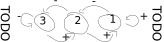
\includegraphics[width=\textwidth]{assets/images/saturating-counter.pdf}
	\caption{Saturating counter}
	\label{fig:saturating-counter}
\end{figure}

In addition to implementing a different update strategy, it might be worth to investigate the use of machine learning or linear programming models as a meta predictor, or even as a prediction algorithm.

\subsection{Final enhancements}
Finally, since some of the implemented algorithms are inherently \tsm{} algorithms rather than prioritisation algorithms, the framework might opt to not execute some test cases at all, whereas now the entire test suite is always executed.\\

\noindent Support for other programming languages and frameworks is possible by implementing new agents. The basic implementation is straightforward to restart the test suite after every executed test case, should test case reordering not be supported natively by the test framework.
\clearpage
%% !TeX root = thesis.tex

\printbibliography[]
\clearpage
%% !TeX = thesis.tex

\cleardoublepage
\addcontentsline{toc}{chapter}{\listfigurename}
\listoffigures
\clearpage
%% !TeX root = thesis.tex

\listoftables
\clearpage
%% !TeX = thesis.tex

\addcontentsline{toc}{chapter}{\lstlistlistingname}
\lstlistoflistings
\clearpage
%% !TeX root = thesis.tex

\begin{appendices}
\appendix
\crefalias{chapter}{appendix}
\addcontentsline{toc}{chapter}{Appendices}
\addtocontents{toc}{\protect\setcounter{tocdepth}{-1}}

\chapter{TravisTorrent queries}
\label{appendix:travistorrent}
\lstinputlisting[caption=TravisTorrent query: Find the amount of failed runs, label=lst:travistorrent-sql1, language=sql]{assets/listings/travistorrent-failed-runs.sql}

\lstinputlisting[caption=TravisTorrent query: Find the probability of consecutive failures,label=lst:travistorrent-sql2, language=sql]{assets/listings/travistorrent-consecutive-failures.sql}

\end{appendices}

\end{document}
